%   \hspace{1.8cm}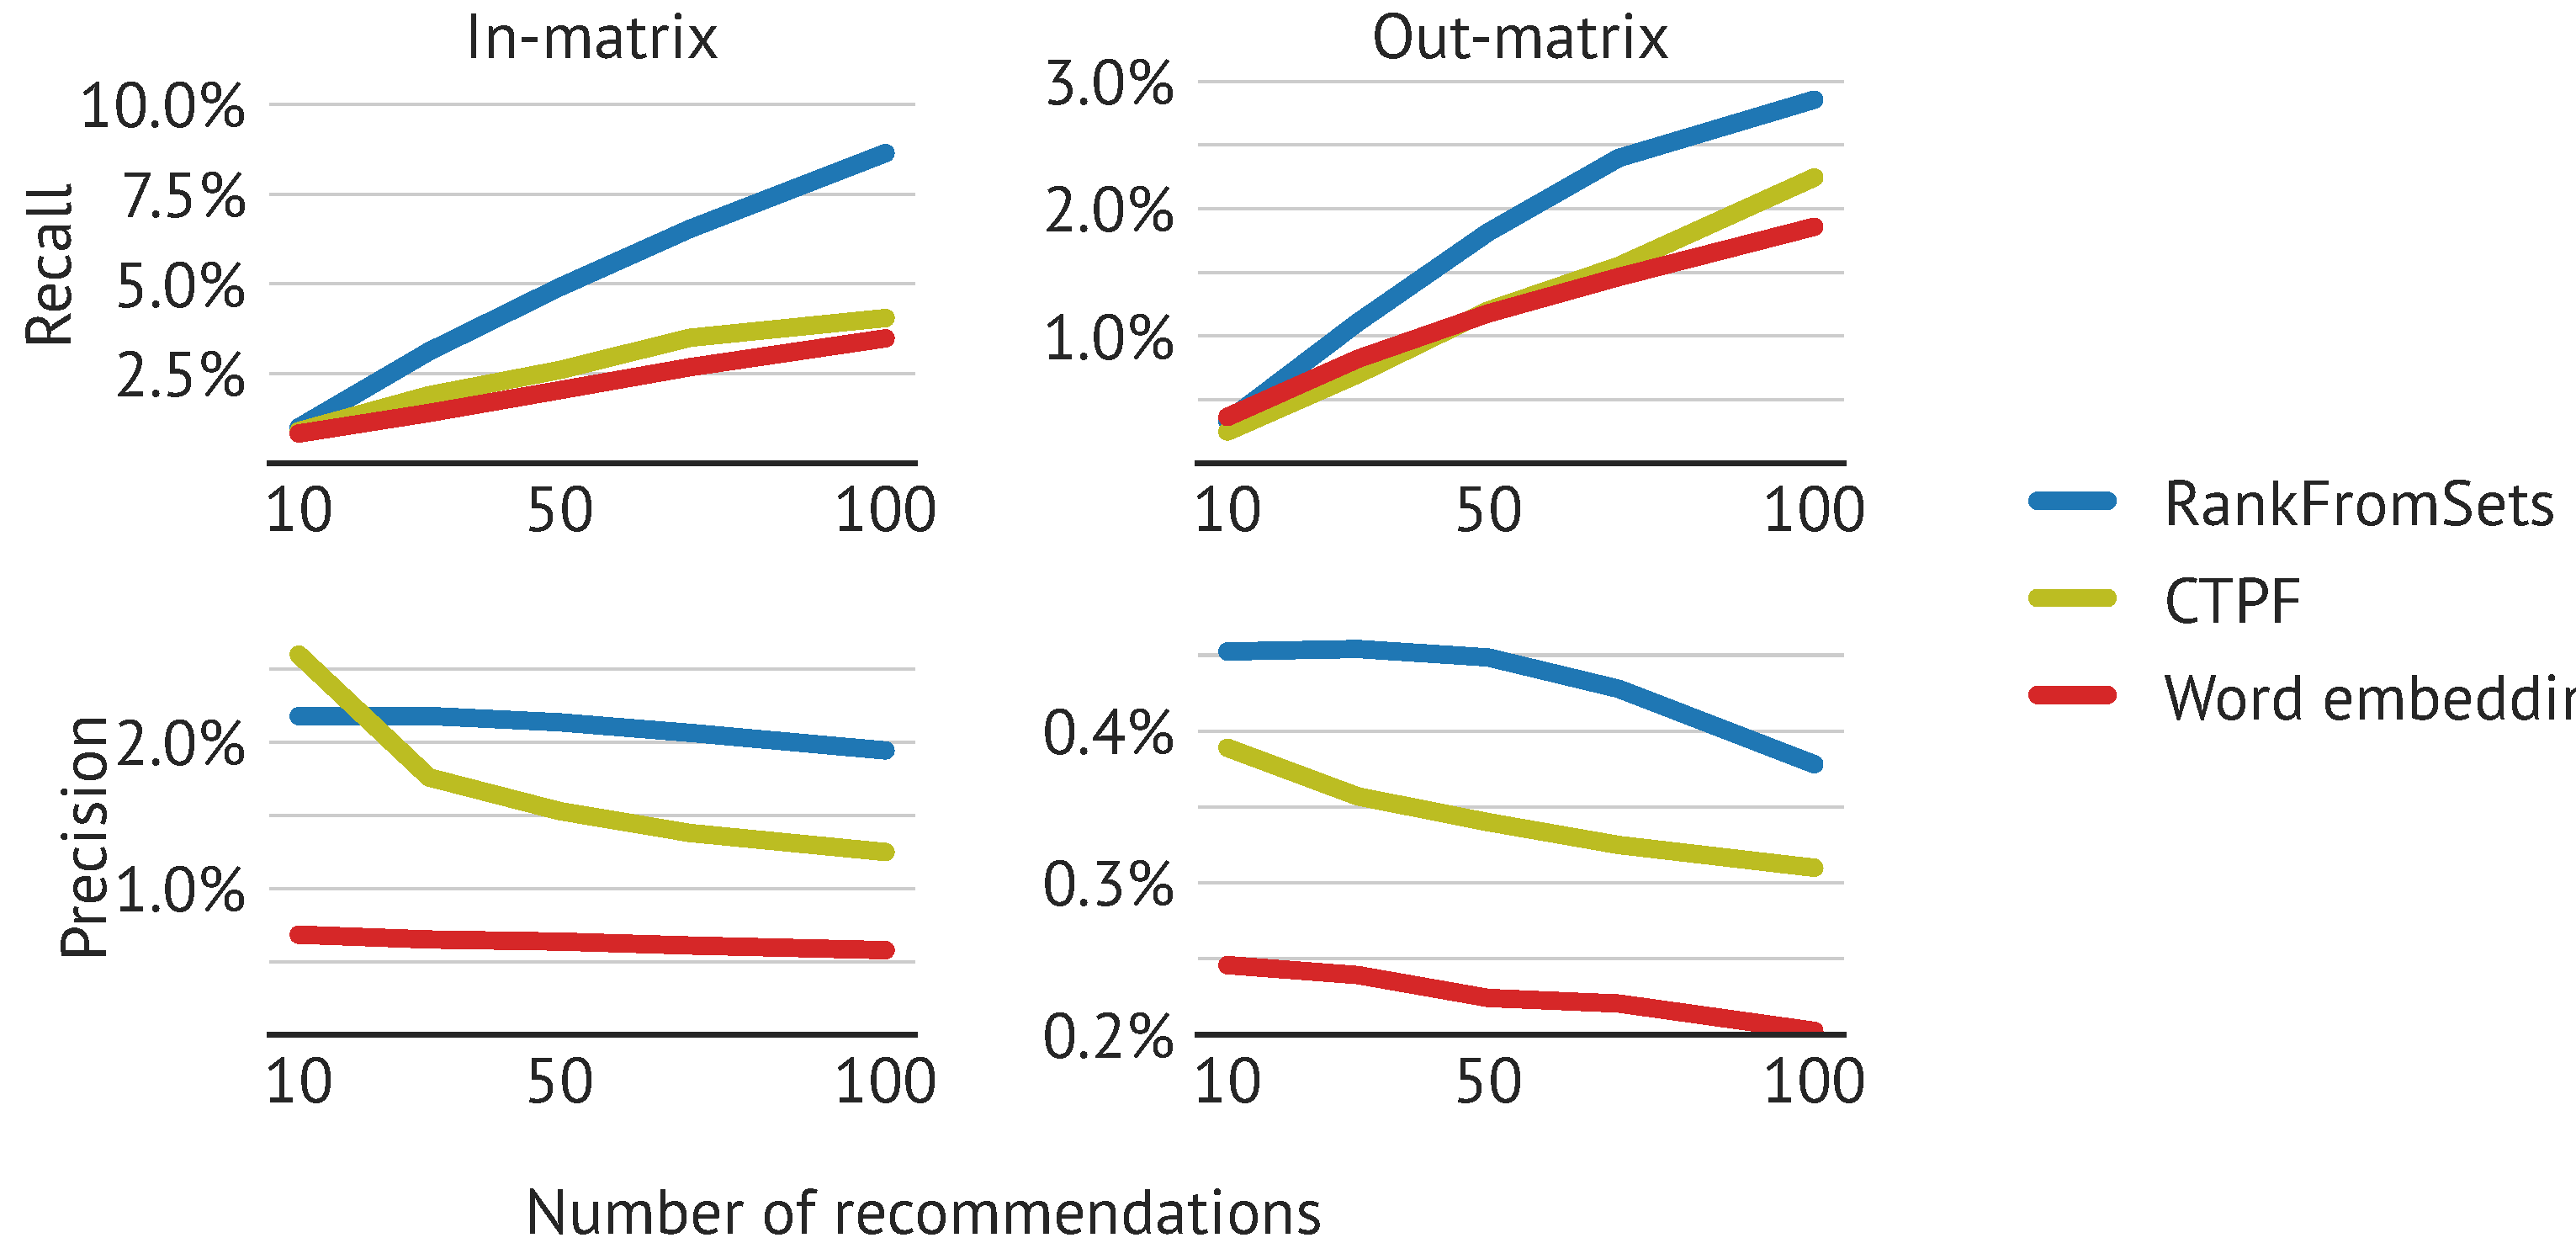
\includegraphics[width=0.7\linewidth]{fig/arxiv}
\newcommand{\mysize}{0.9in}
\newcommand{\mywidth}{0in}
\newcommand{\figwidth}{0.18\linewidth}
\begin{figure*}[t!]
  \centering
  \captionsetup[subfigure]{oneside,margin={-1cm,0cm}}
  \hspace*{\fill}%
  \begin{subfigure}[]{\figwidth}
    \centering
    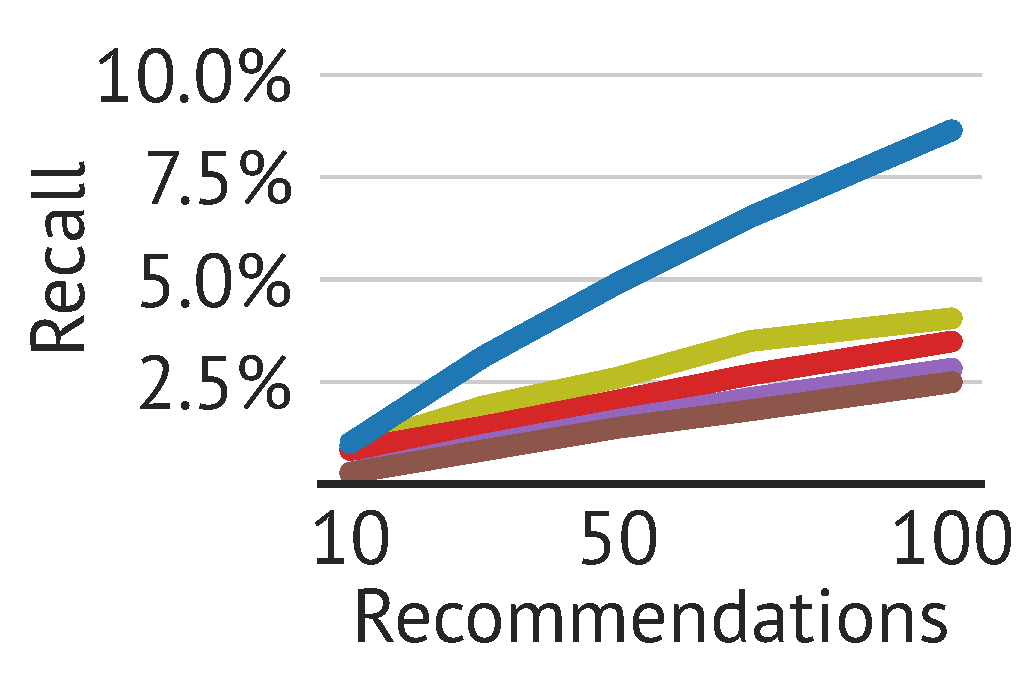
\includegraphics[height=\mysize]{fig/arxiv-in-matrix-recall}
    \caption{In-matrix recall}%
    \label{fig:arxiv-in-recall}%
  \end{subfigure}
  \hfill\hspace{\mywidth}%
  \begin{subfigure}[]{\figwidth}
    \centering
    
\includegraphics[height=\mysize]{fig/arxiv-out-matrix-recall}
    \caption{Out-matrix recall}%
    \label{fig:arxiv-out-recall}%
  \end{subfigure}
  \hfill\hspace{\mywidth}
  \begin{subfigure}[]{\figwidth}
    \centering
    
\includegraphics[height=\mysize]{fig/arxiv-in-matrix-precision}
    \caption{In-matrix precision}%
    \label{fig:arxiv-in-precision}%
  \end{subfigure}
  \hfill\hspace{\mywidth}
  \begin{subfigure}[]{\figwidth}
    \centering
    
\includegraphics[height=\mysize]{fig/arxiv-out-matrix-precision}
    \caption{Out-matrix precision}%
    \label{fig:arxiv-out-precision}%
  \end{subfigure}
  \hfill\hspace{\mywidth}
  \begin{subfigure}[]{0.1\linewidth}
    \centering
    \raisebox{14mm}{
      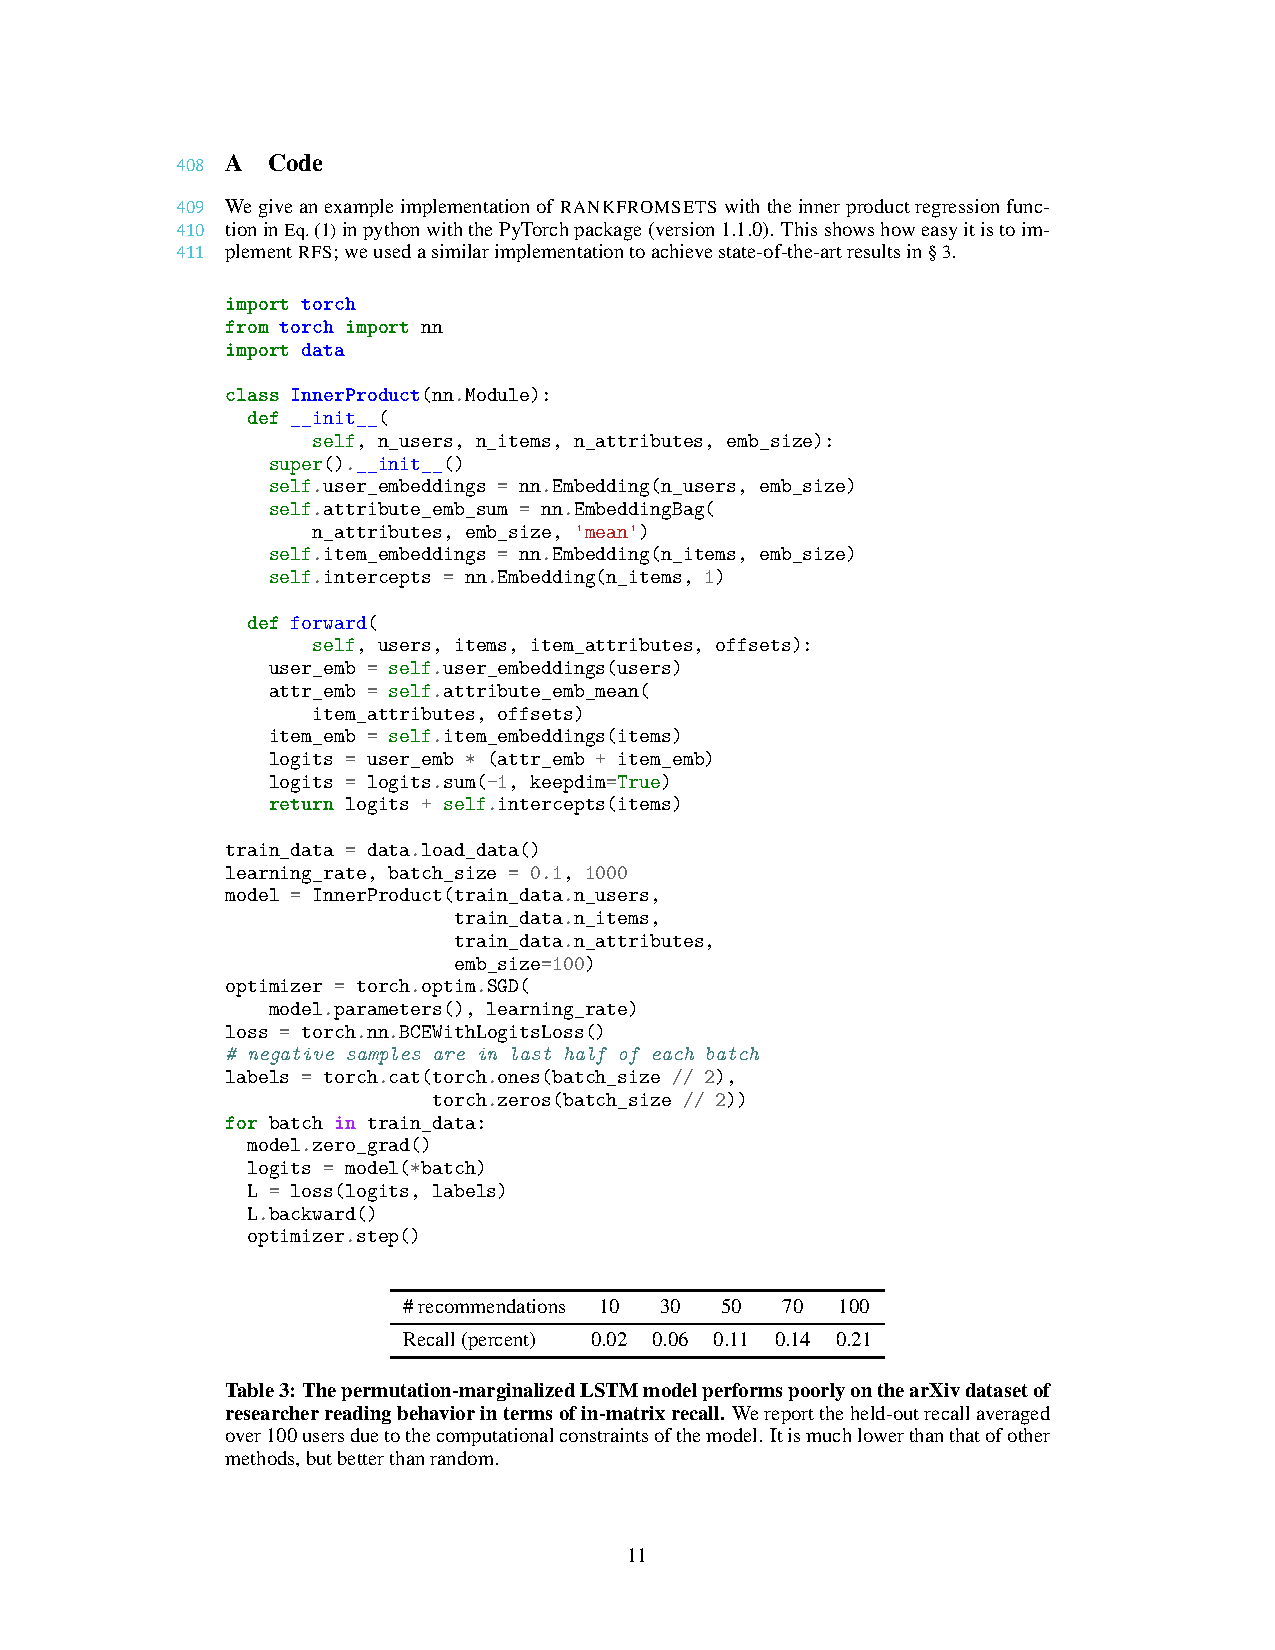
\includegraphics[width=0.9in]{fig/arxiv-legend}
    }
  \end{subfigure}
  \hspace*{\fill}%
  % \vspace{-0.5cm}
  \caption{\label{fig:arxiv-performance} \acrlong{rfs} with the inner
    product regression function in \Cref{eqn:rankfromsets} outperforms
    collaborative topic Poisson factorization (\acrshort{ctpf}, described
    in~\citet{gopalan2014content-based}) and a word embedding model on
    recommending arXiv papers to scientists. In this dataset the items are
    documents and the attributes are the unique words in the abstracts.
    Recommendation performance is evaluated using precision and recall to match
    the evaluation in \citet{gopalan2014content-based}, and these metrics are
    reported on training (in-matrix) documents and cold-start (out-matrix)
    documents with no clicks in the training set. }
\end{figure*}

%%% Local Variables:
%%% mode: latex
%%% TeX-master: "../set_recommendation"
%%% End: